\MDNAME
%%%%%%%%%%%%%%%%%%%%%%%%%%%%%%%%%%%%%%%%%%%%%%%%%%%%%%%%%%%%%%%%%%%%%%%%%%%%%%%
% DO NOT MODIFY THIS FILE
%%%%%%%%%%%%%%%%%%%%%%%%%%%%%%%%%%%%%%%%%%%%%%%%%%%%%%%%%%%%%%%%%%%%%%%%%%%%%%%

\section{Draft: Amazon Web Services}

\label{s:aws} \index{AWS}

\subsection{AWS Products}

Amazon Web Services offers a large number of prodicst that are centered
around their cloud services. These services have grown considerably over
the years from the core offerning realted to virtual machine (EC2) and
datastorage (S3). An overview of them is provided by Amazon in the
following document:

\begin{itemize}
\item
  \url{https://d0.awsstatic.com/whitepapers/aws-overview.pdf}
\end{itemize}

We list the product in screenshots from their Product Web page panel in
Figure \label{F:aws-products}

\begin{figure}
![](images/aws-products-1.png)
![](images/aws-products-2.png)
\caption{AWS Productcs}
\label{F:aws-products}
\end{figure}

Sevice offerings are grouped by categories:

\begin{itemize}
\item
  Compute
\item
  Storage
\item
  Database
\item
  Migration
\item
  Networking and Content Delivery
\item
  Developer Tools
\item
  Management Tools
\item
  Media Services
\item
  Machine Learning
\item
  Analytics
\item
  Security and Identity Compliance
\item
  Mobile Services
\item
  AR and VR
\item
  Application Integration
\item
  Customer Engagement
\item
  Buisiness Productivity
\item
  Desktop and App Streaming
\item
  Internet of Things
\item
  Game Development
\item
  Software
\item
  Aws Core Management
\end{itemize}

Within each category you have several products. When chosing products
form AWS it is best to start with the overview paper and identify
products that can be of benefit to you. For our porpose we focus on the
traditional Compute and Storage offerings.

\subsection{Locations}

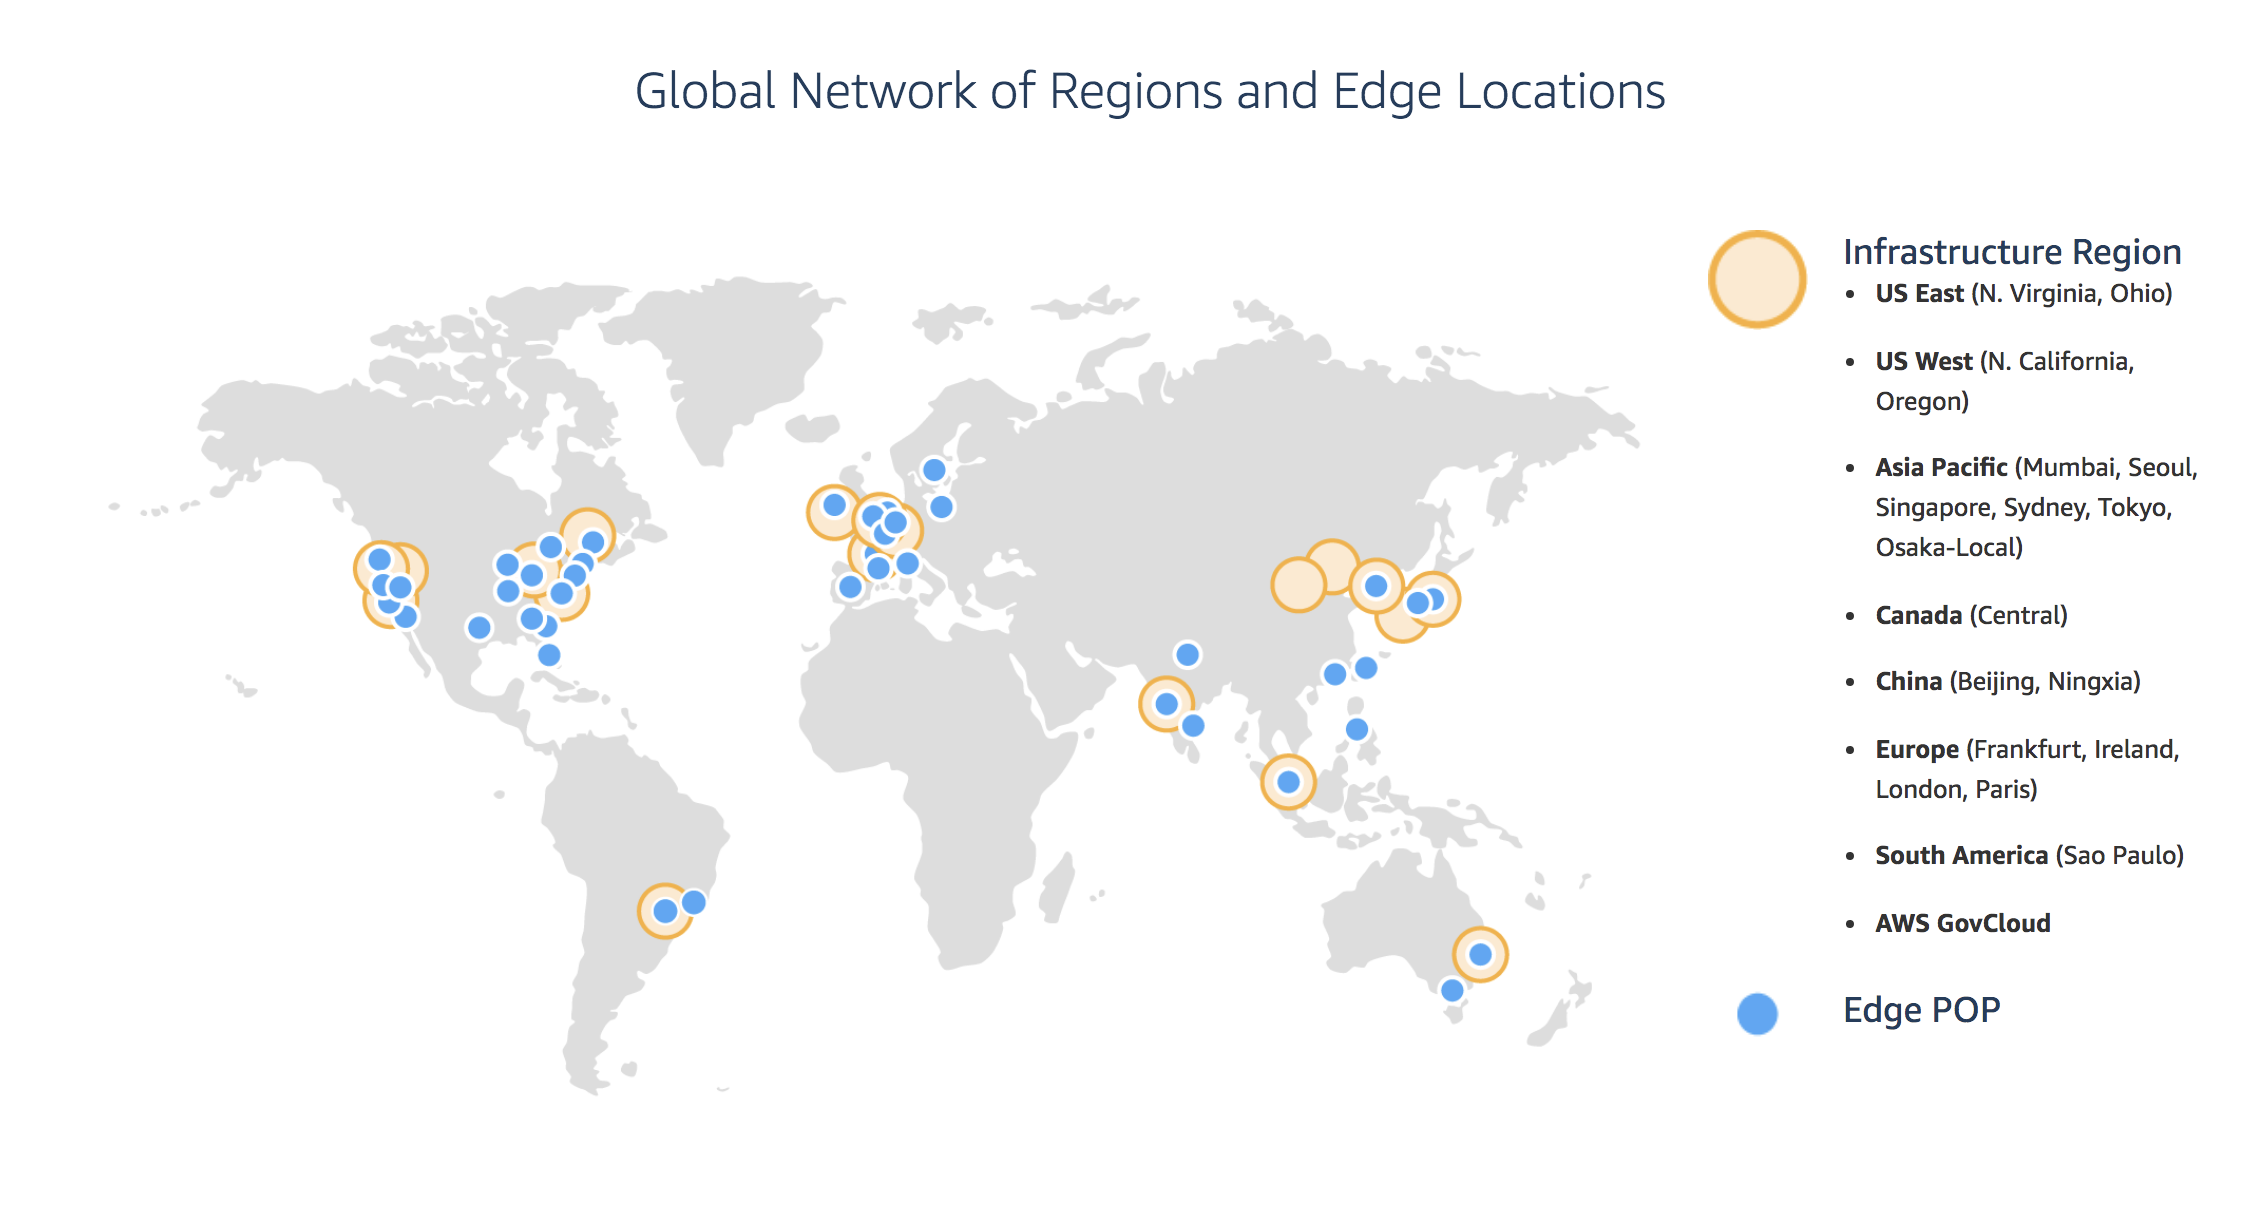
\includegraphics[width=0.8\columnwidth]{images/aws-locations.png}

\subsection{Compute}

AWS offers a number of compute related services.

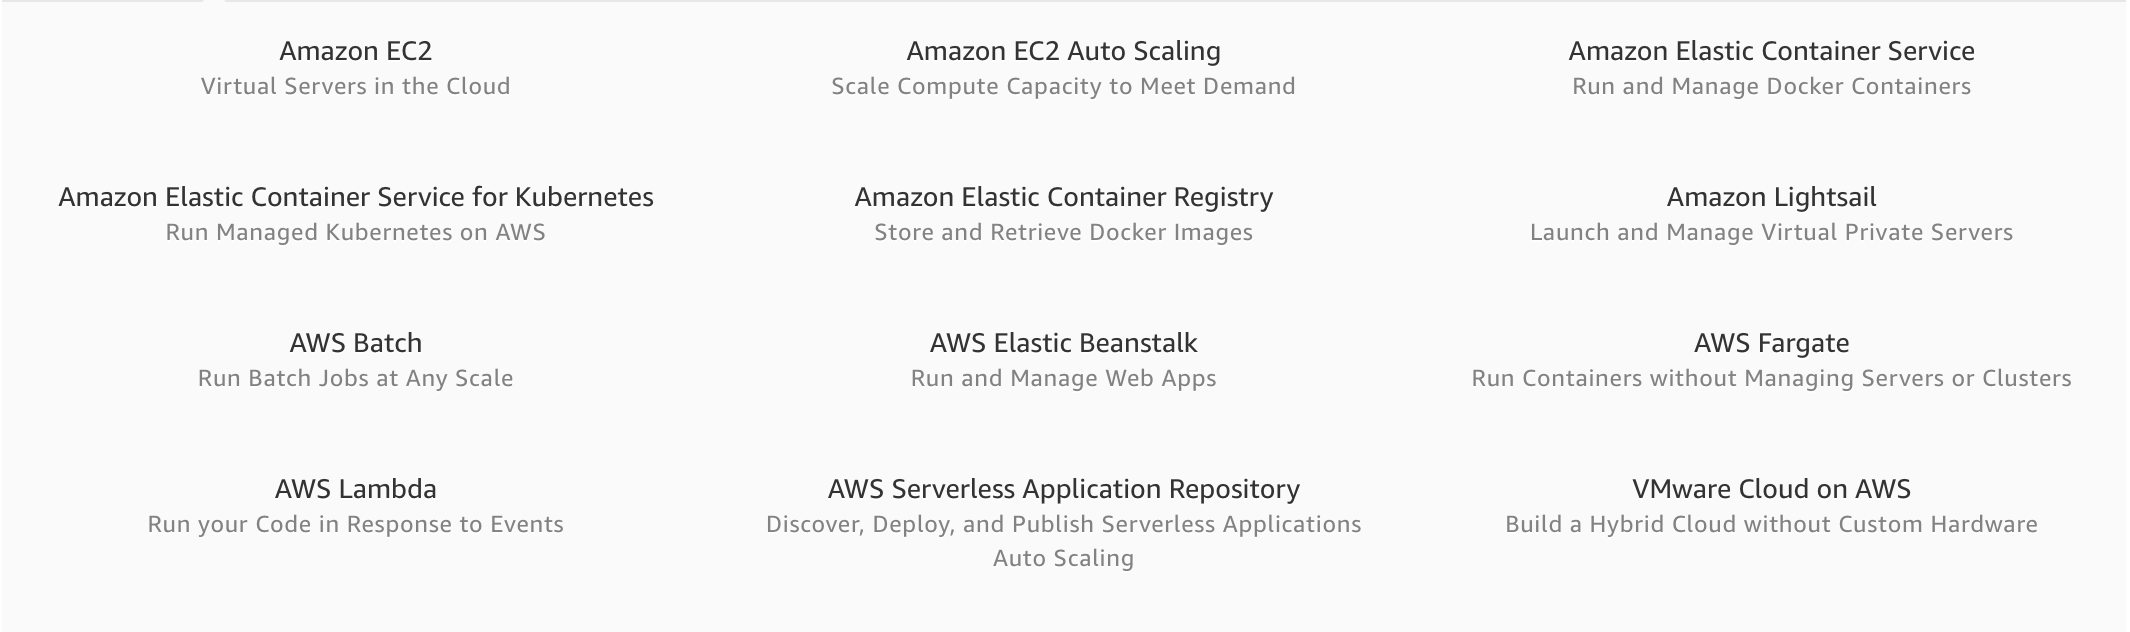
\includegraphics[width=0.8\columnwidth]{images/aws-compute-list.png}

\subsection{Serverless Computing with AWS Lambda}

\url{https://aws.amazon.com/lambda/}

\subsection{Storage}

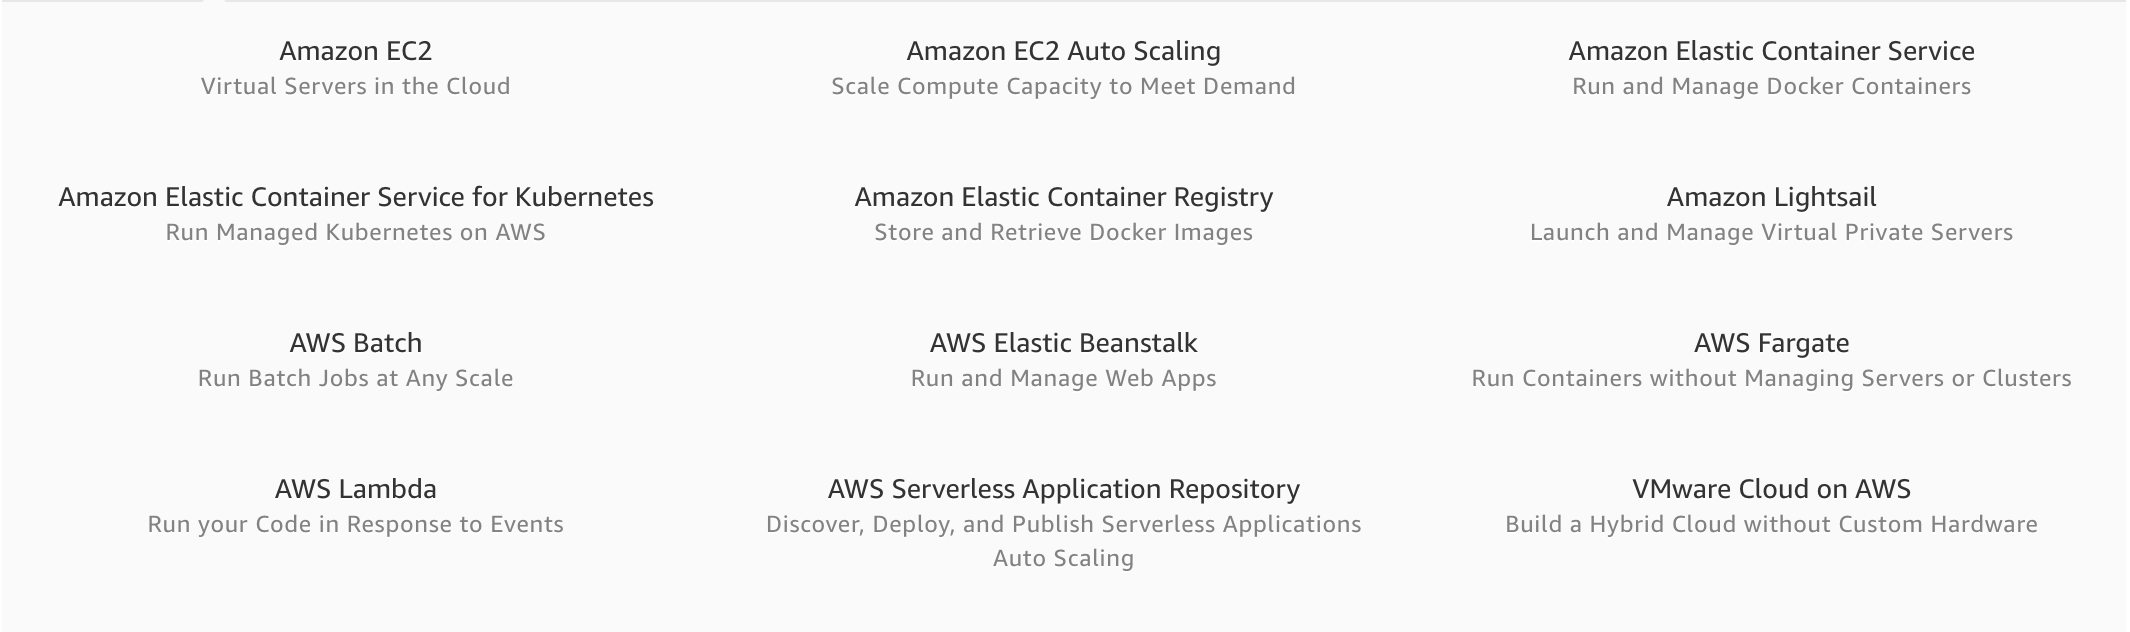
\includegraphics[width=0.8\columnwidth]{images/aws-compute-list.png}

\subsubsection{NoSQL with DynamoDB}

\begin{itemize}
\item
  \url{https://aws.amazon.com/dynamodb/}
\end{itemize}

\subsection{App Integration}

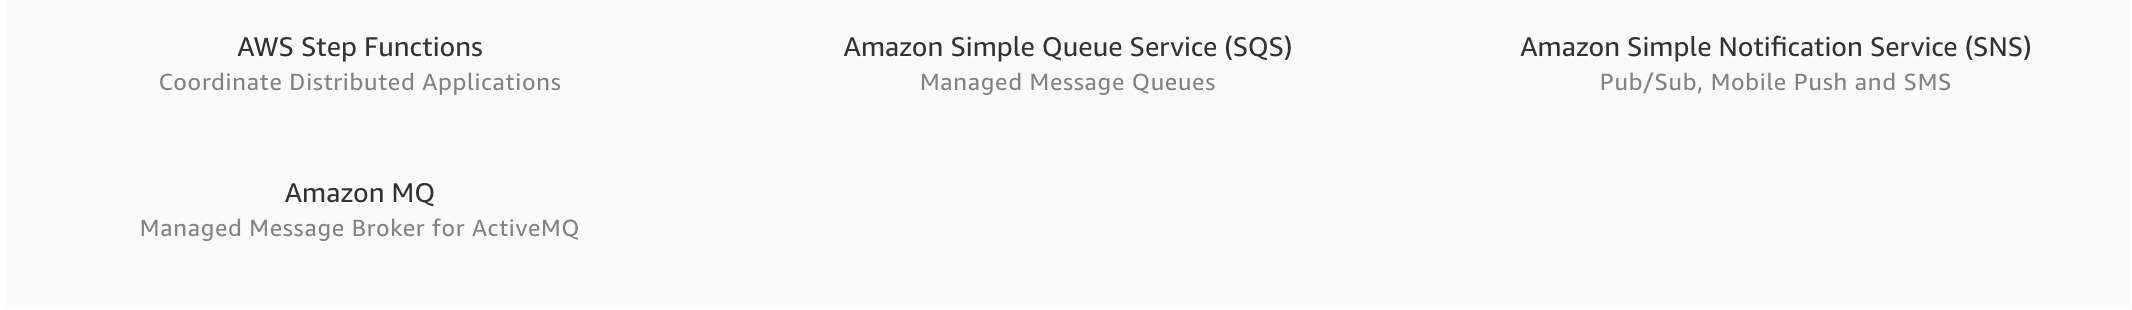
\includegraphics[width=0.8\columnwidth]{images/aws-app-integration.png}

\subsection{Access from the Command Line}

\begin{lstlisting}
aws s3 <Command> [<Arg> ...]
aws ec2 <Command> [<Arg> ...]
\end{lstlisting}

\begin{itemize}
\item
  \url{https://aws.amazon.com/cli/}
\item
  \url{https://docs.aws.amazon.com/cli/latest/reference/}
\item
  EC2:
  \url{https://docs.aws.amazon.com/cli/latest/reference/ec2/index.html}
\item
  S3:
  \url{https://docs.aws.amazon.com/cli/latest/reference/s3/index.html}
\end{itemize}

\subsubsection{S3}

commands: cp, ls, mb, mv, presign, rb, rm, sync, website

\subsection{Access from python}

\subsubsection{libcloud}

\begin{itemize}
\item
  \url{https://libcloud.apache.org/}
\end{itemize}

\subsubsection{Boto}

\begin{itemize}
\item
  \url{https://github.com/boto/boto3}
\end{itemize}

